\chapter{Implementazione}
\label{chap:implementazione}
In questo capitolo si mostra come sono state implementate le funzionalità richieste dalle user stories mostrate nella tabella \ref{tab:user:sto}.
Per ogni funzionalità vedremo quali API sono state create, come sono state documentate attraverso Postman ed il codice utilizzato per realizzarle.

Tutte le rotte relative ai servizi API sono presenti nel file \texttt{/routes.js}, ad esclusione dei servizi relativi alla registrazione e autenticazione di un utente, che si trovano direttamente nel file \texttt{/app.js}.
\section{US-01/03}
Per l'implementazione delle prime tre user stories, che verrano trattate insieme, essendo per lo più simili tra loro, sono stati creati i seguenti servizi:
\begin{lstlisting}[{caption=/routes.js}, style=JavaScriptCode]
module.exports = function(app){
	var List = require('./controllers/lists');
	var Object = require('./controllers/objects');
	var Part = require('./controllers/parts');
	var Option = require('./controllers/options');
	
	app.get('/lists', List.findAll);
	app.get('/lists/:id', List.findById);
	app.post('/lists', List.add);
	app.put('/lists/:id', List.update);
	app.delete('/lists/:id', List.delete);
	
	app.get('/objects/:listid', Object.findAll);
	app.get('/objects/:id', Object.findById);
	app.post('/objects/:listid', Object.add);
	app.put('/objects/:id', Object.update);
	app.delete('/objects/:id', Object.delete);
	
	app.get('/parts/:objectid', Part.findAll);
	app.get('/parts/:id', Part.findById);
	app.post('/parts/:objectid', Part.add);
	app.put('/parts/:id', Part.update);
	app.delete('/parts/:id', Part.delete);
	
	app.get('/options/:partid', Option.findAll);
	app.get('/options/:id', Option.findById);
	app.post('/options/:partid', Option.add);
	app.put('/options/:id', Option.update);
	app.delete('/options/:id', Option.delete);
}
\end{lstlisting}
Come si può vedere, ad ogni operazione CRUD è associata la relativa API, che esegue una specifica funzione presente nel file corrispondente. I file relativi alle suddette funzioni sono contenuti nella cartella \texttt{controllers} e vengono richiamati all'inizio del file \texttt{routes.js}.

Le funzioni sono sufficientemente autoesplicative, ma per chiarezza vengono elencate ed esposte qui di seguito:
\begin{itemize}
	\item \texttt{app.get} si divide in due casi:
	\begin{enumerate}
		\item \texttt{/API} in cui vengono richiesti tutti i Document di una Collection. Nel caso in cui la Collection sia un Object, una Option o una Part, viene passato in input il parametro \texttt{:id} che identifica il Document \emph{parente}.
		\item \texttt{/API/:id} in cui viene passato il parametro \texttt{:id}, per interrogare la Collection nel database MongoDB secondo il criterio di identificazione.
	\end{enumerate}
	\item \texttt{app.post} \\Con questa operazione si aggiunge un Document alla corrispondente Collection. Questo è l'unico caso in cui vanno distinte le Lists dagli altri oggetti. Quando si aggiunge una List tramite metodo POST, non viene passato nessun parametro alla chiamata API. Si noti invece che negli altri casi, durante la medesima operazione, viene sempre passato l'id dell'oggetto \emph{parente}, dell'oggetto ossia a cui fa riferimento il Document che stiamo inserendo.
	\item \texttt{app.put} \\Questa operazione viene usata per modificare un Document già presente in una Collection. Prende in input il parametro \texttt{:id} per poter ritrovare il giusto oggetto su cui eseguire un \emph{update}.
	\item \texttt{app.delete} \\Infine l'operazione \emph{delete} si usa per eliminare un Document specifico, che viene identificato, come sopra, prendendo in input il parametro \texttt{:id}. 
\end{itemize}

Di seguito prendiamo in esame il controller relativo agli Objects per analizzare le relative funzioni, seguite dalla relativa documentazione realizzata con Postman:
\begin{lstlisting}[{caption=/controllers/objects.js}, style=JavaScriptCode]
var mongoose = require('mongoose'),
Object = require('../app/schema.js').model('Object');

exports.findAll = function(req, res){
	var listid = req.params.listid;
	Object.find({'_list': listid},function(err, docs) {
		return res.send(docs);
	});
};

exports.findById = function(req, res){
	var id = req.params.id;
	Object.findOne({'_id': id, '_list': listid},function(err, docs) {
		return res.send(docs);
	});
};

exports.add = function(req, res) {
	var listid = req.params.listid;
	Object.create({"nome": req.body.nome, "descrizione": req.body.descrizione, 
	"_list": listid}, function (err, docs) {
		if (err) return console.log(err);
		return res.send(docs);
	});
};

exports.update = function(req, res) {
	var id = req.params.id;
	var updates = req.body;
	console.log(id);
	Object.update({"_id":id}, req.body,
	function (err, numberAffected) {
		if (err) return console.log(err);
		console.log('Updated %d Lists', numberAffected);
		return res.sendStatus(202);
	});
};

exports.delete = function(req, res) {
	var id = req.params.id;
	Object.remove({'_id':id},function(result) {
		return res.send(result);
	});
};
\end{lstlisting}

L'interfacciamento con il database è gestito tramite mongoose, di cui viene importata la dipendenza all'inizio del file.
La prima funzione è \texttt{findAll}, che prende in input, attraverso i parametri presenti nella request, l'id della List a cui l'Object è associato. Viene quindi eseguita la funzione \texttt{.find} di mongoose sulla Collection Objects, filtrando per l'id appena passato, e quello che si avrà come risposta sarà una callback, che conterrà un messaggio di errore in caso di fallimento, o i Document richiesti in caso di successo. A questo punto il server invia la risposta tramite la funzione \texttt{res.send}, includendo i risultati dell'interrogazione appena effettuata sul database. La funzione \texttt{findById} è molto simile alla precedente, pertanto non verrà spiegata nuovamente.
\begin{figure}[h]
	\centering
	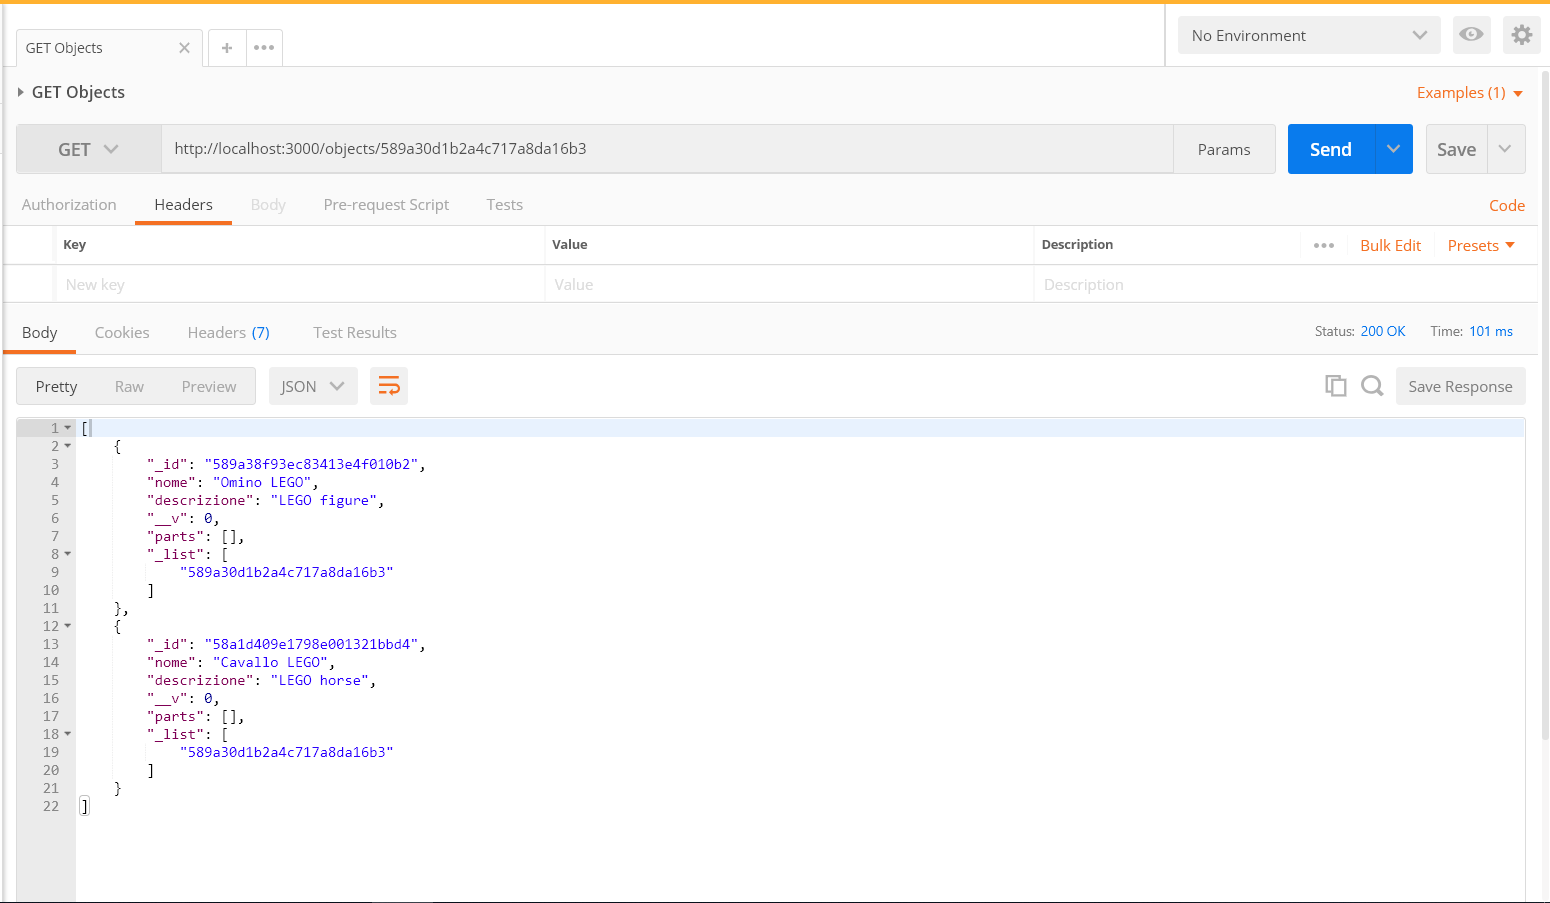
\includegraphics[scale=0.42]{Immagini/get_objects.png}
	\caption{Documentazione get /objects/:id}
\end{figure}

La funzione \texttt{add} inserisce un nuovo Object Document nella sua Collection, solo dopo però averlo inizializzato inserendo l'id della List a cui fa riferimento nell'attributo \texttt{\_list}, il nome (preso dal \emph{body} della richiesta HTTP) nell'attributo \texttt{nome} e la descrizione nel corrispondente attributo. I parametri nome e descrizione sono stati inseriti dall'utente negli appositi campi presenti nella pagina di visualizzazione degli Objects, e vengono trasmessi al server attraverso la richiesta HTTP POST.
\begin{figure}[h]
	\centering
	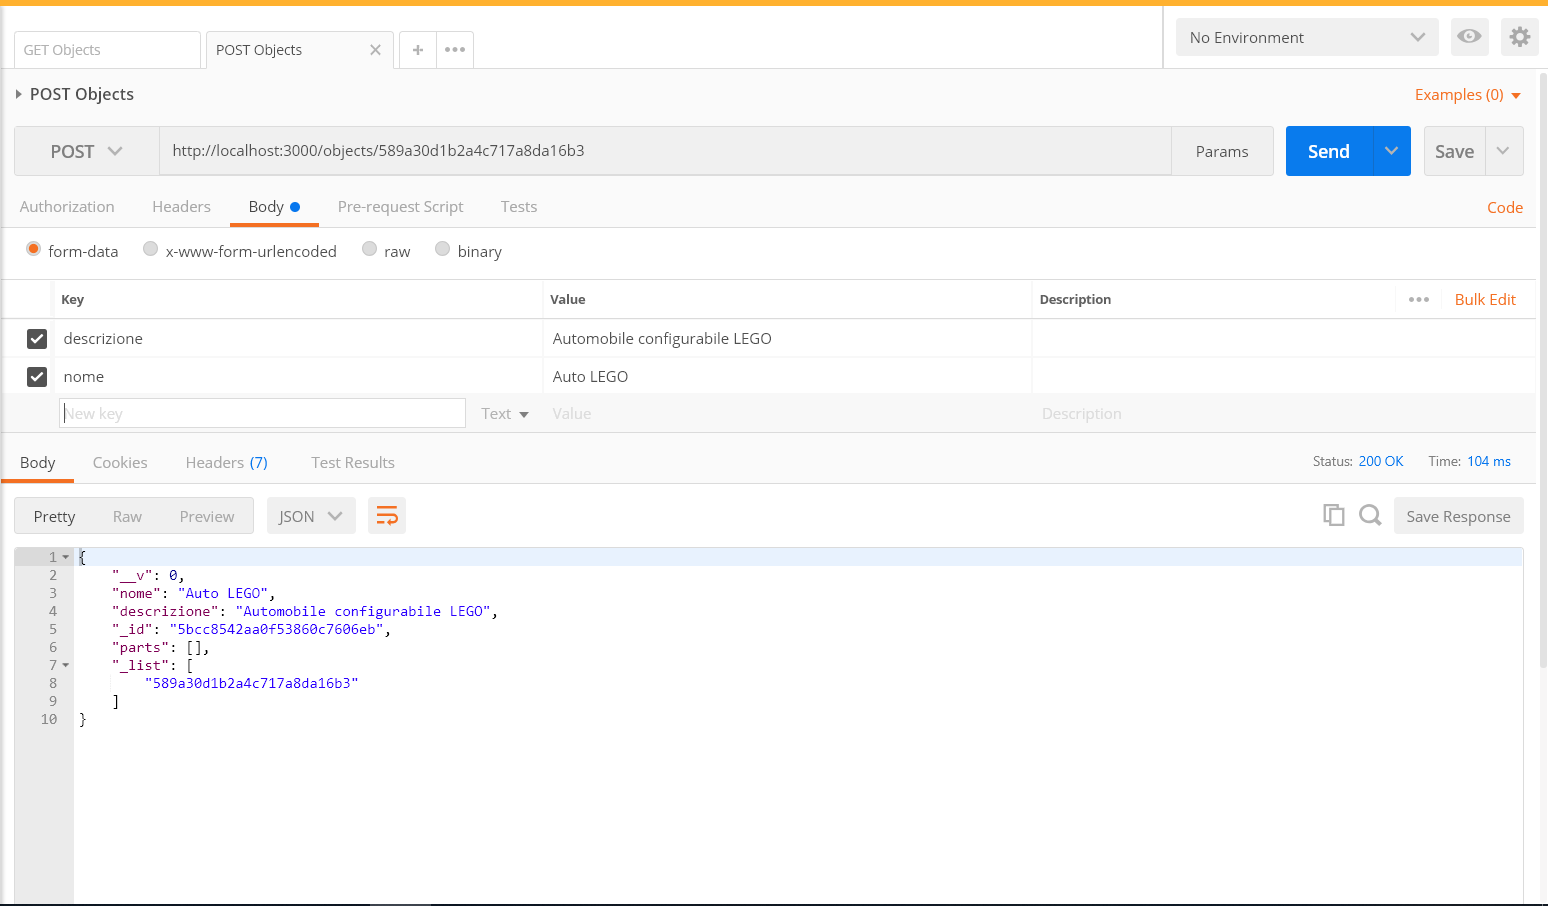
\includegraphics[scale=0.42]{Immagini/post_objects.png}
	\caption{Documentazione post /objects/:id}
\end{figure}

L'ultima funzione è \texttt{delete}. Questa rimuove l'Object cercandolo attraverso il suo \texttt{id}. La funzione non necessita di alcun parametro aggiuntivo.
\begin{figure}[h]
	\centering
	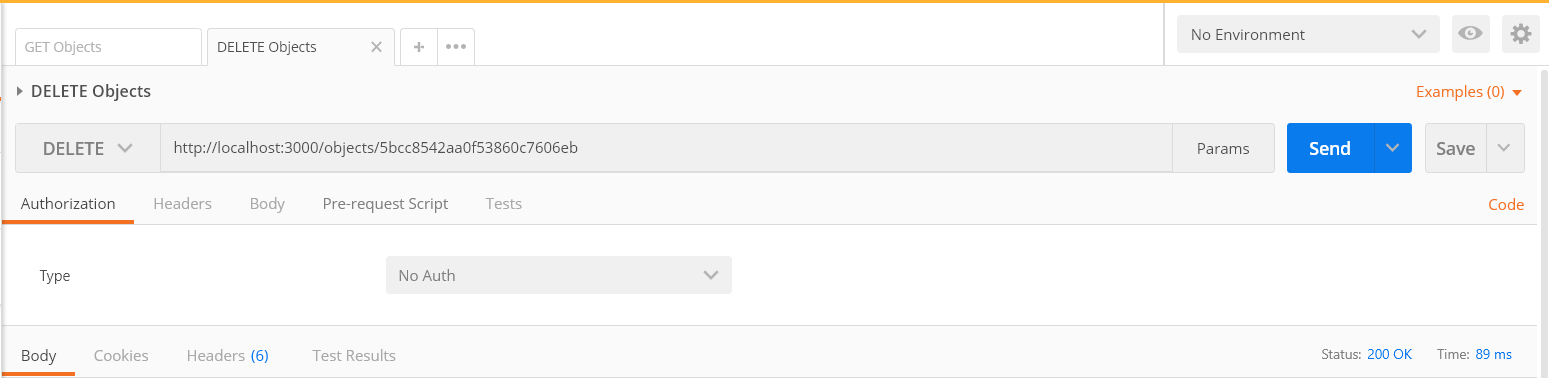
\includegraphics[scale=0.42]{Immagini/delete_objects.png}
	\caption{Documentazione delete /objects/:id}
\end{figure}

Le funzioni si comportano in modo analogo, o comunque come spiegato sopra, con gli altri tipi di oggetti in unicam-product-editor.
Per quanto riguarda la funzione di visualizzazione dei documenti richiesta dalle user stories dalla 01 alla 03, è stata sviluppata una applicazione single-page in AngularJS, che andremo a vedere nella US-05.
\section{US-04}
La user story 04 richiede di avere un endpoint che restituisca la forma JSON di un oggetto 3D da visualizzare.

Per implementare questa funzione, è stata creata una chiamata API apposita, contenuta nel file del server \texttt{app.js}.

\begin{lstlisting}[{caption=shape API}, style=JavaScriptCode]
app.get('/shape/:id', cors(corsOptions), function(req, res){
	var search = req.params.id;
	converted(req, search, res);
});
\end{lstlisting}
Come possiamo vedere dallo snippet di codice qui sopra, la API rimanda alla apposita funzione converted, situata in \texttt{/app/converted.js}.

\begin{lstlisting}[{caption=/app/converted.js}, style=JavaScriptCode]
coll.find({"_id" : mongodb.ObjectId(search)}).toArray(function(err, docs) {
	if (err){
		console.log('error in db');
		res.end();
		return;
	}
	else if (docs.length == '0'){
		console.log('No files found');
		res.send('No files found');
	}
	else{
		res.send(docs);
	}
});
\end{lstlisting}
Lo scopo della funzione è quello di trovare nella Collection Shapes il documento JSON corrispondente a quello dell'id richiesto. In questa particolare Collection, i JSON non seguono uno Schema come nel caso degli altri oggetti, ma vengono conservati così come sono, essendo questi il risultato della conversione dei file .obj. Così quando il server risponderà, non lo farà usando uno stato risultante di una richiesta HTTP, ma lo farà inviando il JSON vero e proprio. Grazie a questo tipo di risposta, unicam-product-viewer avrà il suo enpoint a cui agganciarsi per prendere le forme 3D da visualizzare nella propria interfaccia.
\begin{figure}[h]
	\centering
	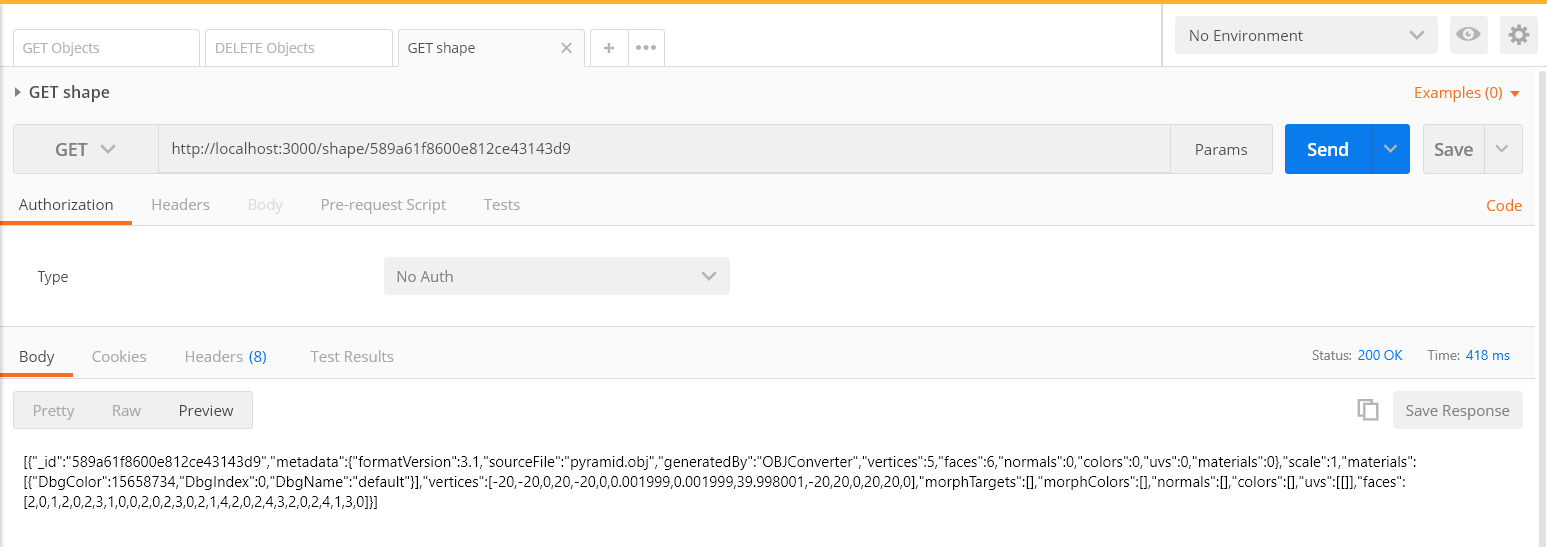
\includegraphics[scale=0.42]{Immagini/get_shape.png}
	\caption{Documentazione get /shape/:id}
\end{figure}
\section{US-05}
Questa User story richiede di sviluppare una \emph{single-page application} che serva da client per l'utente. L'applicazione in questione è stata realizzata usando AngularJS\index, un framework web principalmente sviluppato da Google. La tecnologia che usa AngularJS è di tipo Single Page Application (SPA); una SPA viene eseguita all’interno di una singola pagina HTML: tutte le risorse necessarie alla sua esecuzione vengono caricate dinamicamente ed aggiunte al DOM (Document Object Model) della pagina corrente. In altre parole, all’interno di una singola pagina vengono caricate viste diverse in base all’interazione dell’utente con la pagina stessa. Questo approccio consente di creare applicazioni responsive che si avvicinano al funzionamento delle applicazioni desktop.

La root del client sviluppato in AngularJS è interamente contenuta nella cartella \texttt{/public}, ed oltre al file principale, \texttt{/public/app.js}, sono presenti le cartelle dei principali componenti usati dal framework, come i \emph{controllers}, le \emph{directives}, i \emph{services}, la cartella \texttt{vendors} che ospiterà in locale le librerie usate in unicam-product-editor, come la già citata jQuery, la cartella \texttt{partials} che conterrà le pagine HTML richieste come risorse e la cartella \texttt{stylesheets} che racchiude i file .css, ossia i fogli di stile, usati dall'applicazione.

Nel file principale, \texttt{/public/app.js} sono indicati tutti gli stati usati dalla libreria \texttt{\$stateProvider} e in cui il client può trovarsi in fase di navigazione.
\begin{lstlisting}[{caption=/public/app.js}, style=JavaScriptCode]
$stateProvider
.state('home', {
	url: '/',
	controller: 'HomeCtrl',
	templateUrl: '/static/partials/home.html'
})
\end{lstlisting}
\begin{figure}[h]
	\centering
	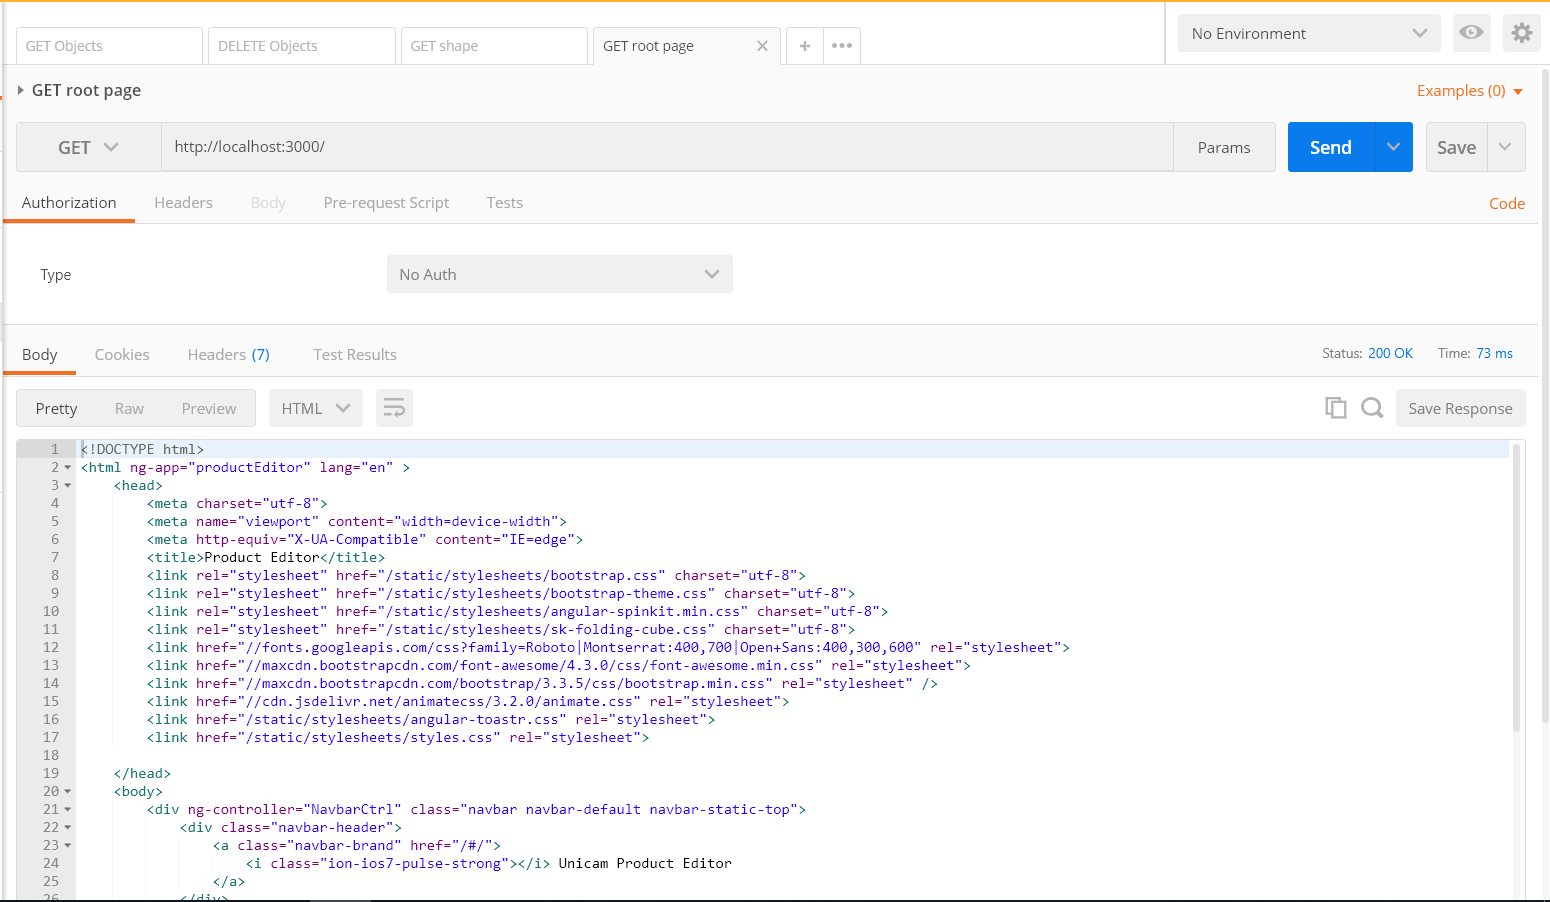
\includegraphics[scale=0.42]{Immagini/get_root.png}
	\caption{Documentazione get /}
\end{figure}

Quello appena esposto, ad esempio, è lo stato relativo alla route principale. Non appena si digiterà l'URL \texttt{http://localhost:3000/} nel caso il server sia ospitato in locale, o \texttt{http://unicam-product-editor.herokuapp.com/} nel caso in cui si sfrutti l'applicazione rilasciata su Heroku, AngularJS riconoscerà di trovarsi nello stato di \emph{home}, e invierà al client come risposta la pagina HTML indicata nella proprietà \texttt{templateUrl}, \texttt{/static/partials/home.html}, e a questa associerà il relativo controller, \texttt{HomeCtrl}. Tutti i controller sono contenuti nella cartella \texttt{/public/controllers}.

I controller servono per eseguire le operazioni lato client, per inizializzare le richieste HTTP a seguito di un'azione. Andiamo per esempio ad analizzare il controller relativo alla pagina web delle Lists:
\begin{lstlisting}[{caption=/public/controllers/lists.js}, style=JavaScriptCode]
angular.module('productEditor')
.controller('ListsCtrl', function($scope, $http, $location, toastr){
	$http.get('/lists')
	.success(function(docs) {
		$scope.lists = docs;
	})
	.error(function(err) {
		toastr.error('Error! Something went wrong');
	});
	...
\end{lstlisting}
le istruzioni esposte qui sopra fanno sì che, non appena il client richiede la pagina web delle Lists, il controller avvia la richiesta HTTP \texttt{/lists}, tramite la quale si richiedono tutte le Lists presenti nella Collection Lists. La risposta viene messa nella variabile \texttt{\$scope.lists}, e viene poi renderizzata tramite AngularJS nella pagina HTML
\begin{lstlisting}[{caption=/public/partials/lists.html}, style=JavaScriptCode]
...
<tr ng-repeat="list in lists">
	<td ng-hide="list.edit">{[{list.nome}]}</td>
		<td ng-show="list.edit"><input type="text" ng-model="list.nome"></td>
...
\end{lstlisting}
La direttiva \texttt{ng-repeat} ripete l'elemento \emph{lista} contenuto nella variabile \texttt{lists} dello \texttt{\$scope}, esponendone la proprietà \texttt{nome} tante volte quante sono le istanze degli elementi ripetuti nella variabile.
\begin{figure}[h]
	\centering
	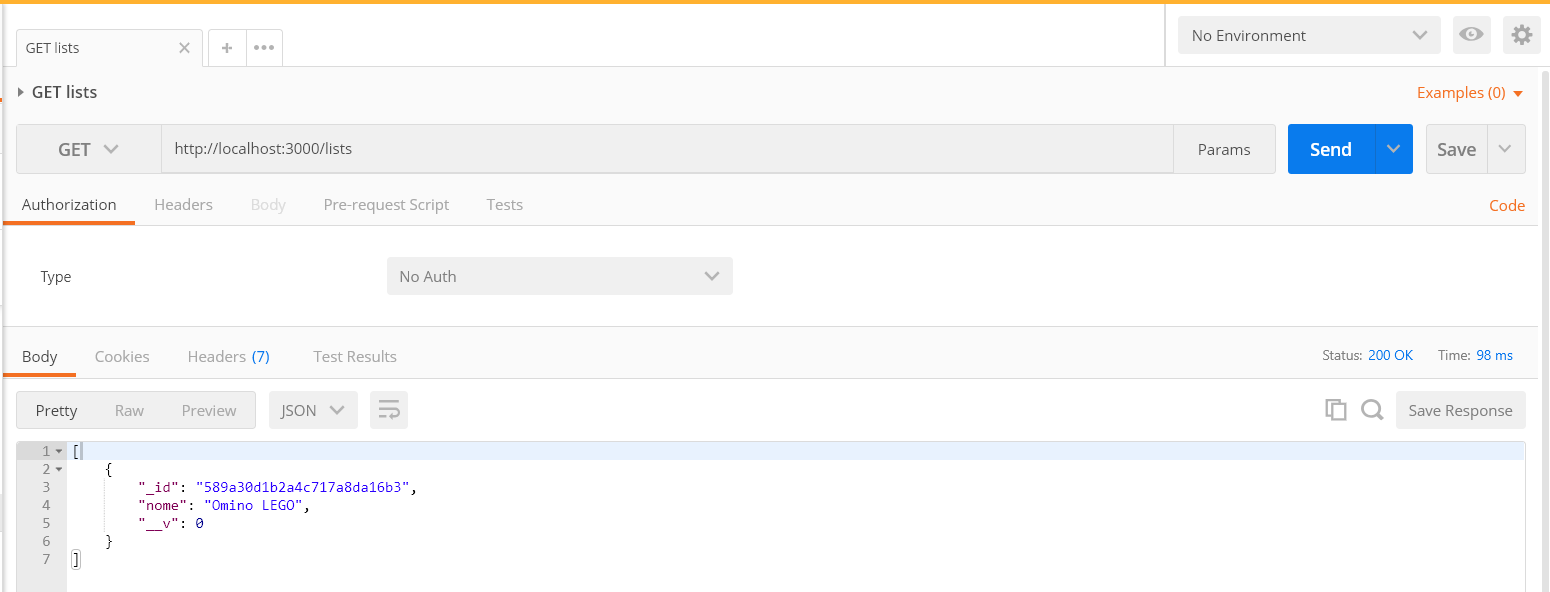
\includegraphics[scale=0.42]{Immagini/get_lists.png}
	\caption{Documentazione get /lists}
\end{figure}

La breve panoramica appena esposta spiega quindi il percorso che seguono le informazioni dalla fase di richiesta del client, all'elaborazione della risposta dal server, fino alla gestione della risposta ricevuta dal client.

\section{US-06}
La prossima user story richiede che il processo di caricamento della forma 3D avvenga in modo sincrono, e che non sia bloccante. Abbiamo già trattato il modo in cui il long polling sia stato implementato nel client nel capitolo \ref{chap:long_polling}, pertanto andremo a vedere soltanto il codice lato server.

Nel processo di caricamento di una forma 3D, la prima richiesta HTTP che viene effettuata è una richiesta POST, che contiene nel body il file .obj della forma che si vuole caricare. A questo punto la API chiama la funzione upload dal file \texttt{/app/upload.js}.
\begin{lstlisting}[{caption=/app/upload.js}, style=JavaScriptCode]
var express = require('express'),
	fileUpload = require('express-fileupload'),
	bodyParser = require('body-parser'),
	app = express(),
	mongodb = require('mongodb'),
	path = require('path'),
	http = require('http'),
	fs = require('fs'),
	path = require('path'),
	convert = require('./convert');

app.use(express.static('app'));
app.use(fileUpload());

module.exports = function upload(req, res) {
	var filename = req.files.file.name;
	
	var ext = path.extname(filename);
	if (ext != '.obj'){
		console.log('File is not .obj');
		res.redirect(505, 'Error in file inserted');
	}
	else {
		var target_path = './public/tmp/' + filename;
		req.files.file.mv(target_path,function (err){
			if (err) throw err;
			console.log('File uploaded!');
			convert(req, filename, res);
		});
	};
};
\end{lstlisting}
La funzione di upload salva il file 3D .obj nel percorso \texttt{/public/tmp} con lo stesso nome con cui viene caricato. A questo punto viene chiamata a sua volta la funzione \texttt{convert}, localizzata nella stessa directory del file \texttt{upload.js}.
\begin{lstlisting}[{caption=/app/convert.js}, style=JavaScriptCode]
var express = require('express'),
	app = express(),
	PythonShell = require('python-shell'),
	bodyParser = require('body-parser'),
	fs = require('fs'),
	path = require('path'),
	upload = require('./upload'),
	readjsonfile = require('./readjsonfile');

module.exports = function convert (req, filename, res){
	filename = './public/tmp/' + filename;
	var truncate = filename.substr(0, filename.lastIndexOf('.')) || filename;
	var options = {
	mode: 'text',
	scriptPath: './scripts',
	args: ['-i', filename, '-o', truncate + '.json']};
	
	PythonShell.run('converter.py', options, function (err, results) {
		if (err){
		throw err;
	}
	console.log('results: %j', results);
	filename = truncate + '.json';
	res.setHeader('Content-Type', 'application/json');
	res.send(JSON.stringify(filename, null, 3));
	});
};
\end{lstlisting}
Il file appena caricato viene convertito in JSON attraverso lo script Python \texttt{converter.py} contenuto nella cartella \texttt{/scripts}, che come detto in precedenza fa parte della libreria Three.js. Per essere eseguito, lo script viene passato come parametro alla funzione \texttt{run} della libreria \texttt{PythonShell}. Una volta finita l'operazione di conversione, si invia il file JSON in risposta come endpoint, tramite la funzione \texttt{JSON.stringify}.
L'ultima operazione che viene eseguita è quella di inserimento del file JSON nel database, che avviene tramite la chiamata HTTP \texttt{/insert}. La API corrispondente rimanda il body dell'endpoint (quindi il JSON da inserire) alla funzione \texttt{readjsonfile}, che dopo aver inserito il JSON nel database, elimina i file temporanei creati durante l'intero processo.
\begin{lstlisting}[{caption=/app/readjsonfile.js}, style=JavaScriptCode]
var express = require('express'),
	app = express(),
	bodyParser = require('body-parser'),
	fs = require('fs'),
	path = require('path'),
	mongoose = require('mongoose'),
	mongodb = require('mongodb')
	convert = require('./convert');

var id;
var screenid;
var path;

module.exports = function readjsonfile(res, data, db){
	var coll = mongoose.connection.db.collection('shapes');
	coll.save(data);
	path = "./public/tmp/" + data.metadata.sourceFile;
	id = data._id;
	screenid = 'ID:' + id;
	console.log(screenid);
	fs.unlinkSync(path);
	path = (path.substr(0, path.lastIndexOf('.')) || path) + '.json';
	fs.unlinkSync(path);
	res.setHeader('Content-Type', 'application/json');
	res.send(JSON.stringify('insert success', null, 3));
}
\end{lstlisting}

Va da sé che tutte queste operazioni devono essere eseguite consecutivamente ed in un certo ordine, e per questo il processo di upload usato in unicam-product-editor entra in contrasto con la natura di Node.js che, essendo un sistema event-driven, esegue le operazioni in modo asincrono.
La chiave che fa sì che le operazioni di questo processo siano eseguite nel giusto ordine sono le callback: durante il passaggio da una sequenza di istruzioni all'altra, nei punti chiave, le funzioni vengono chiamate usando le callback, pertanto l'esecuzione di queste istruzioni non si conclude finché non finisce il processo successivo, e finché quindi non si riceve il risultato attraverso la callback, formando una catena di operazioni eseguite in modo sincrono.
\section{US-07}
La ultima user story prevede che un nuovo utente all'interno di unicam-product-editor possa registrarsi, o che un utente già registrato possa effettuare un login.

Per questa funzionalità in unicam-product-editor è stato usato Satellizer\index{Satellizer}, un modulo aggiuntivo creato per AngularJS di autenticazione basato sui token. Con questo sistema l'utente è in grado di registrarsi ed eseguire il login sia con una semplice autenticazione basata su username e password che con l'autenticazione da terze parti (OAuth 1.0 e OAuth 2.0), come Google, Facebook, LinkedIn, Twitter, Instagram, GitHub ed altri. Nel nostro progetto è stata implementata l'autenticazone attraverso Google e Facebook, oltre a quella con indirizzo e-mail e password.

L'implementazione di questo modulo prevede i seguenti step (l'esempio qui riportato è quello dell'autenticazione Google):
\begin{enumerate}
	\item Installazione tramite il comando \texttt{npm install satellizer}.
	\item Importazione del Javascript nel client attraverso la pagina HTML, usando il tag \texttt{<script src="satellizer.js"></script>}.
	\item Importazione del modulo nel controller principale della Single Page Application
	\begin{lstlisting}[style=JavaScriptCode]
	$authProvider.google({
		clientId: 'Google Client ID'
	});
	\end{lstlisting}
	\item Implementazione del sistema di chiamate HTTP nel controller della pagina di autenticazione
	\begin{lstlisting}[style=JavaScriptCode]
	$scope.authenticate = function(provider) {
		$auth.authenticate(provider);
	};
	\end{lstlisting}
	\item Configurazione della chiamata HTTP specifica per ogni opzione di autenticazione
	\begin{lstlisting}[style=JavaScriptCode]
	$authProvider.google({
		url: '/auth/google',
		authorizationEndpoint: 'https://accounts.google.com/o/oauth2/auth',
		redirectUri: window.location.origin,
		requiredUrlParams: ['scope'],
		optionalUrlParams: ['display'],
		scope: ['profile', 'email'],
		scopePrefix: 'openid',
		scopeDelimiter: ' ',
		display: 'popup',
		oauthType: '2.0',
		popupOptions: { width: 452, height: 633 }
	});
	\end{lstlisting}
	\item Nel caso di autenticazione OAuth come lo è Google, ottenere le Chiavi OAuth nella sezione sviluppatori di Google (Google+ APIs).
\end{enumerate}
Una volta configurato correttamente, si può usare Satellizer all'interno di un qualsiasi controller della nostra applicazione web usando il modulo \texttt{\$auth} con una delle funzioni messe a disposizione, come \texttt{login} per effettuare il login, \texttt{signup} per registrarsi o \texttt{isAuthenticated} per controllare la presenza di un token attivo di autenticazione.  
\begin{figure}[h]
	\centering
	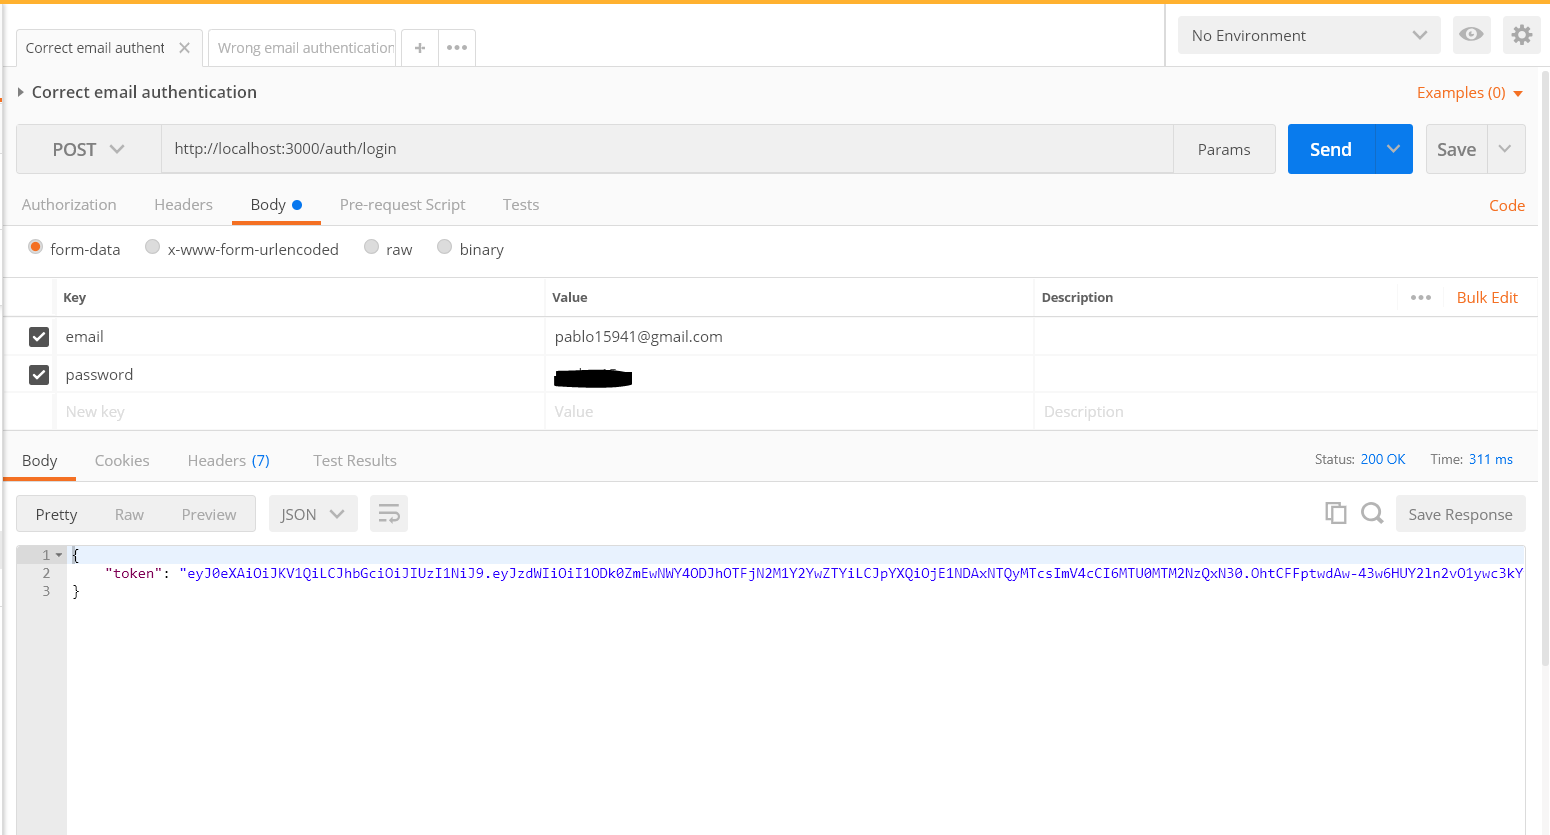
\includegraphics[scale=0.42]{Immagini/correct_auth.png}
	\caption{Documentazione post /auth/login}
\end{figure}
In caso di login corretto, il server invierà come risposta il token di autenticazione.
\begin{figure}[h]
	\centering
	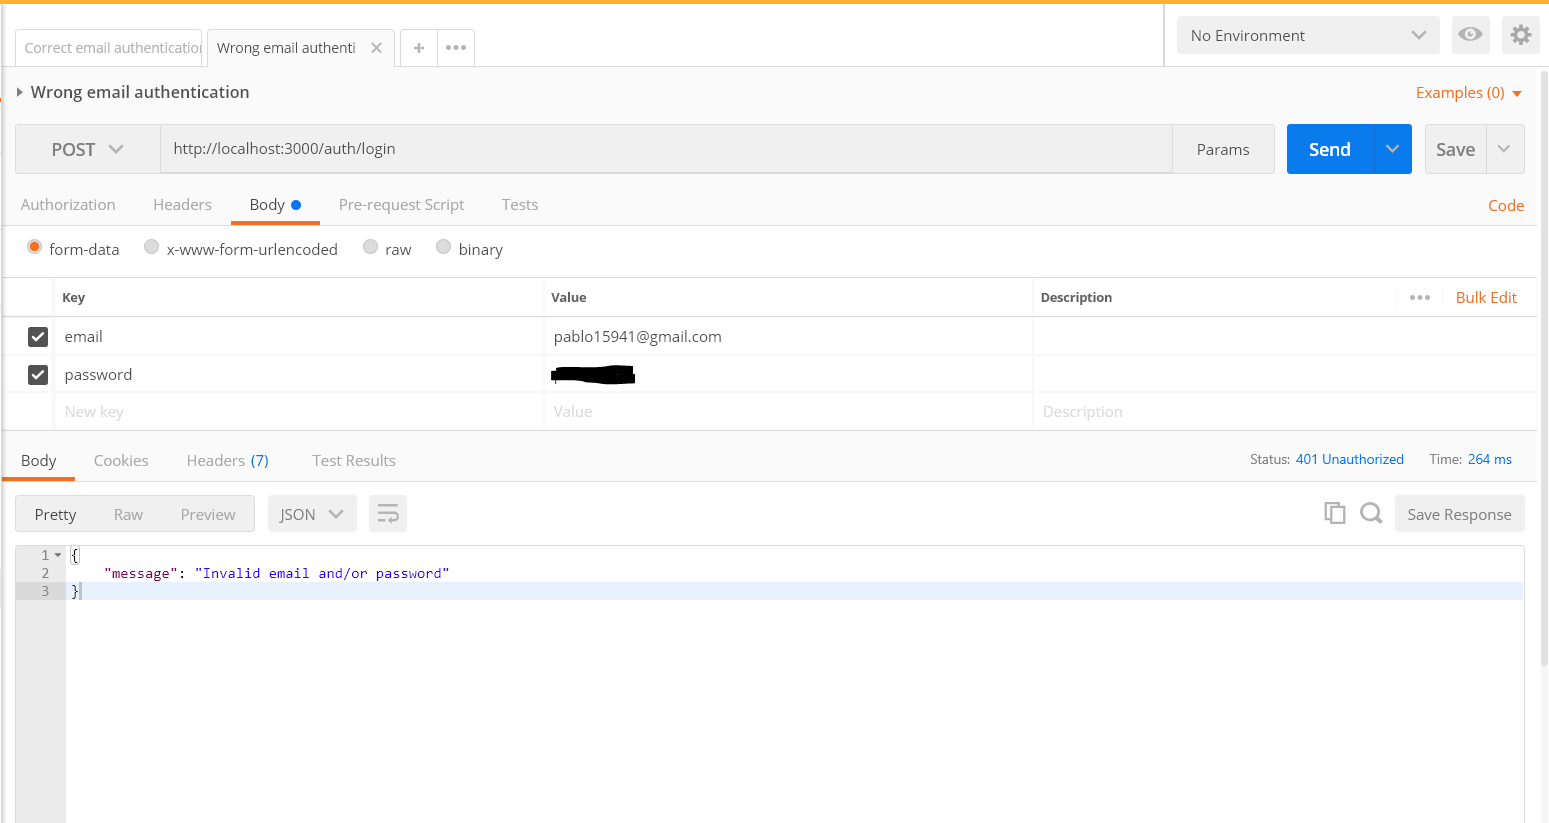
\includegraphics[scale=0.42]{Immagini/wrong_auth.png}
	\caption{Documentazione post /auth/login sbagliato}
\end{figure}
In caso contrario, la risposta del server sarà un messaggio di errore con stato \texttt{401, Unauthorized}.